\documentclass{article}
\usepackage{latexsym}
\usepackage{amssymb}
\usepackage{graphicx}
\usepackage{gensymb}
\usepackage[margin=1.2in]{geometry}
\usepackage{float}
\usepackage{wrapfig}
\usepackage{amsthm}
\usepackage{blkarray}
\usepackage{amsmath}
\usepackage{mathtools}
\usepackage{tikz}

\usepackage{framed}
\usepackage{fancyhdr}
\setcounter{page}{0}
\fancypagestyle{plain}{%
\pagestyle{fancy}
\fancyhf{}
\rhead{Tom Goodman}
\lhead{\leftmark}
\chead{Introduction to AI - Exercise I}
\cfoot{\thepage} 
\renewcommand{\footrulewidth}{2pt}}
\pagestyle{plain}
\newcounter{thrmcount}[section]

\usepackage{graphicx}
    \graphicspath{ {/home/txg523/Desktop} }

\newenvironment{thrm}
	{\begin{leftbar}\noindent\ignorespaces\textbf{Theorem \arabic{section}.\arabic{thrmcount}.}\par\noindent\ignorespaces}		
	{\end{leftbar}\stepcounter{thrmcount}\noindent\ignorespaces}
\newenvironment{lem}
	{\begin{leftbar}\noindent\ignorespaces\textbf{Lemma \arabic{section}.\arabic{thrmcount}.}\par\noindent\ignorespaces}		
	{\end{leftbar}\stepcounter{thrmcount}\noindent\ignorespaces}
\newenvironment{nthrm}[1]	
	{\begin{leftbar}\noindent\ignorespaces\textbf{Theorem \arabic{section}.\arabic{thrmcount}.} \textit{(#1)}\par\noindent\ignorespaces}
	{\end{leftbar}\stepcounter{thrmcount}\noindent\ignorespaces}
\newenvironment{nlem}[1]
	{\begin{leftbar}\noindent\ignorespaces\textbf{Lemma \arabic{section}.\arabic{thrmcount}.} \textit{(#1)}\par\noindent\ignorespaces}
	{\end{leftbar}\stepcounter{thrmcount}\noindent\ignorespaces}
\newenvironment{defn}
	{\begin{leftbar}\noindent\ignorespaces\textbf{Definition.}\par\noindent\ignorespaces}
	{\end{leftbar}\noindent\ignorespaces}
\newenvironment{nproof}
	{\begin{proof}}
	{\newline\end{proof}\noindent\ignorespaces}
\newenvironment{prop}
	{\begin{leftbar}\noindent\ignorespaces\textbf{Proposition \arabic{section}.\arabic{thrmcount}.}\par\noindent\ignorespaces}		
	{\end{leftbar}\stepcounter{thrmcount}\noindent\ignorespaces}
\newenvironment{fact}
	{\begin{leftbar}\noindent\ignorespaces\textbf{Fact \arabic{section}.\arabic{thrmcount}.}\par\noindent\ignorespaces}		
	{\end{leftbar}\stepcounter{thrmcount}\noindent\ignorespaces}
\newenvironment{crl}
	{\begin{leftbar}\noindent\ignorespaces\textbf{Corollary \arabic{section}.\arabic{thrmcount}.}\par\noindent\ignorespaces}		
	{\end{leftbar}\stepcounter{thrmcount}\noindent\ignorespaces}	
\newenvironment{ex}[1]
	{\begin{leftbar}\noindent\ignorespaces\textbf{Example.} (\textit{#1})\par\noindent\ignorespaces}
	{\end{leftbar}\noindent\ignorespaces}
\newenvironment{exa}
	{\begin{leftbar}\noindent\ignorespaces\textbf{Example.}\par\noindent\ignorespaces}
	{\end{leftbar}\noindent\ignorespaces}
\newcommand\ddfrac[2]{\frac{\displaystyle #1}{\displaystyle #2}}
\newcommand{\appropto}{\mathrel{\vcenter{
  \offinterlineskip\halign{\hfil$##$\cr
    \propto\cr\noalign{\kern2pt}\sim\cr\noalign{\kern-2pt}}}}}
\title{Goodman's Approximation}
\author{Tom Goodman}
\date{}
\begin{document}
\begin{titlepage}
	\begin{flushleft}
		\vspace*{1cm}
		\Huge
		\textbf{Introduction to AI - Exercise I} \\
		\vspace*{1cm}
		\Large
		\textbf{Tom Goodman} \\
	\end{flushleft}
\end{titlepage}
\newpage
\section{Graph}
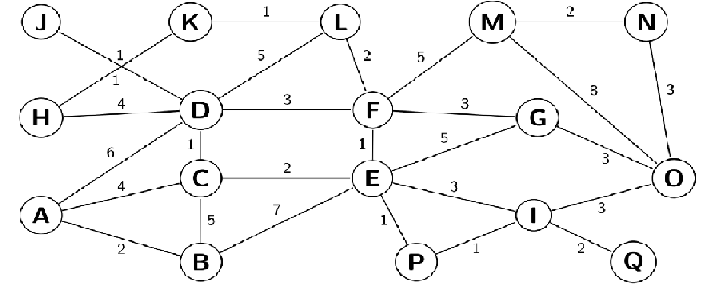
\includegraphics{IntroToAIE1Graph.png}
\section{Question One}
\subsection{Brief}
\textit{For this exercise ignore the path costs. Perform Depth-First-Search to find a path from
A to O. Assume that nodes are expanded in alphabetic order. Write down carefully the
values in your data structures Explored and Frontier as well as the search tree. $[30\% - 30\ marks]$}
\subsection{Answer - Data Structures}
\begin{center}
    \begin{tabular}{ l | c}
    
    \hline
    \textbf{Frontier} & \textbf{Explored}\\
    
    \hline
    $[A_{1}]$ &  [ ] \\ \hline 
    $[B_{2}, C_{3}, D_{4}]$ & $[A_{1}]$ \\ \hline
    $[C_{5}, E_{6}, C_{3}, D_{4}]$ & $[A_{1}, B_{2}]$ \\ \hline    
    $[D_{7}, E_{8}, E_{6}, C_{3}, D_{4}]$ & $[A_{1}, B_{2}, C_{5}]$ \\ \hline
    $[F_{9}, H_{10}, J_{11}, L_{12}, E_{8}, E_{6}, C_{3}, D_{4}]$ & $[A_{1}, B_{2}, C_{5}, D_{7}]$ \\ \hline
    $[E_{13}, G_{14}, M_{15}, H_{10}, J_{11}, L_{12}, E_{8}, E_{6}, C_{3}, D_{4}]$ & $[A_{1}, B_{2}, C_{5}, D_{7}, F_{9}]$ \\ \hline
    $[G_{16}, I_{17}, P_{18}, G_{14}, M_{15}, H_{10}, J_{11}, L_{12}, E_{8}, E_{6}, C_{3}, D_{4}]$ & $[A_{1}, B_{2}, C_{5}, D_{7}, F_{9}, E_{13}]$ \\ \hline
    $[O_{18}, I_{17}, P_{18}, G_{14}, M_{15}, H_{10}, J_{11}, L_{12}, E_{8}, E_{6}, C_{3}, D_{4}]$ & $[A_{1}, B_{2}, C_{5}, D_{7}, F_{9}, E_{13}, G_{16}]$ \\ \hline
        
    \end{tabular}

\newpage
\subsection{Answer - Tree}    
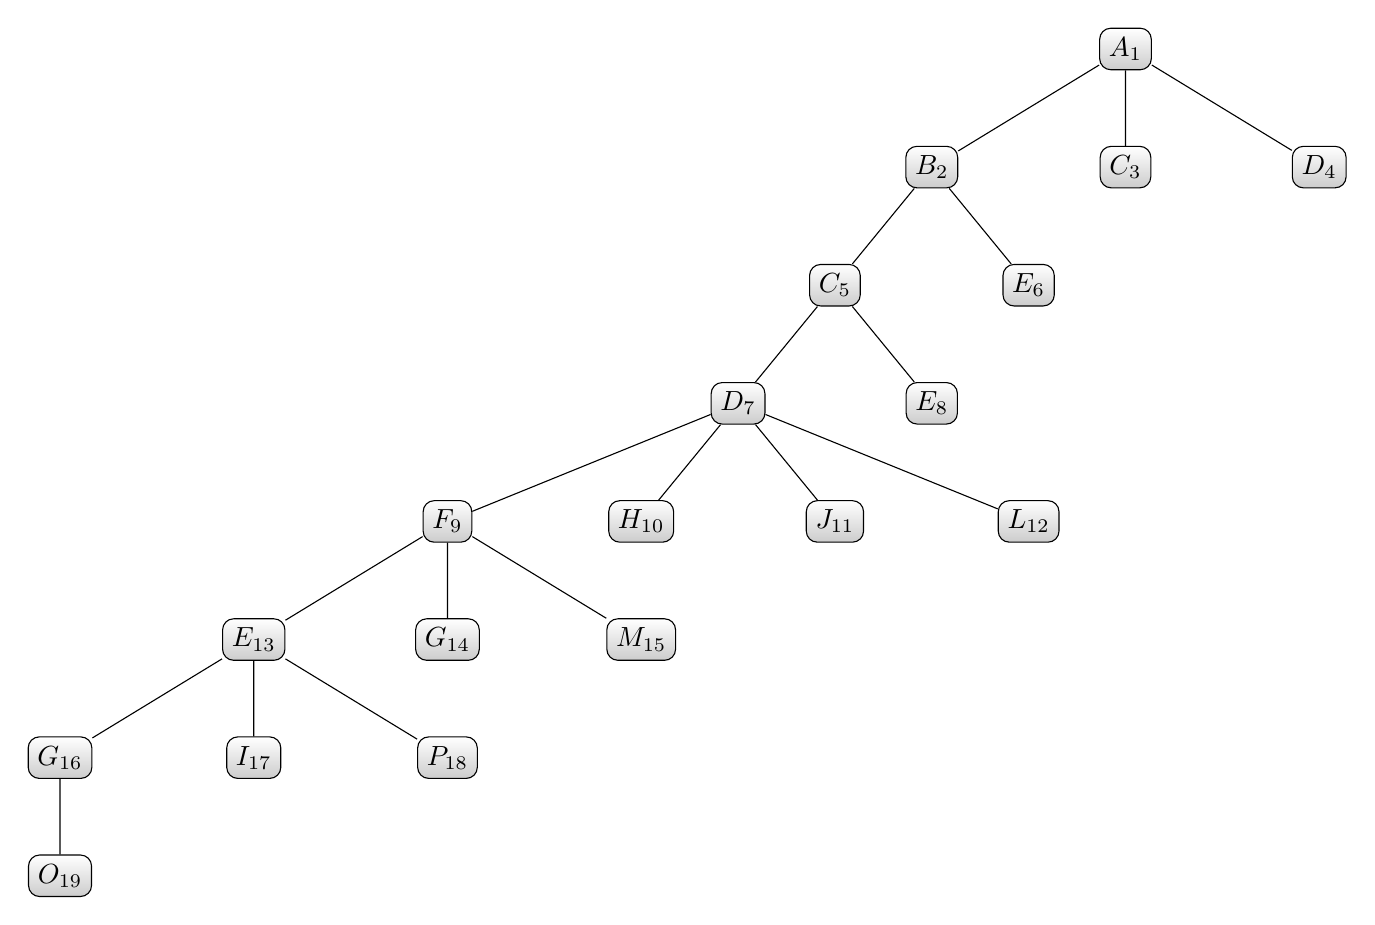
\begin{tikzpicture}[sibling distance=7em, every node/.style = {shape=rectangle, rounded corners, draw, align=center, top color = white, bottom color = black!20}]]
    \node{$A_{1}$}
        child{ node{$B_{2}$}
            child{ node{$C_{5}$}
                child{ node{$D_{7}$}
                    child{ node{$F_{9}$}
                        child{ node{$E_{13}$}
                            child{ node{$G_{16}$}
                                child{ node{$O_{19}$}}}
                            child{ node{$I_{17}$}}
                            child{ node{$P_{18}$}}}                            
                        child{ node{$G_{14}$}}
                        child{ node{$M_{15}$}}}
                    child{ node{$H_{10}$}}
                    child{ node{$J_{11}$}}
                    child{ node{$L_{12}$}}}
                child{ node{$E_{8}$}}}
            child{ node{$E_{6}$}}}
        child{ node{$C_{3}$}}
        child{ node{$D_{4}$}};
    \end{tikzpicture} \\
  
\subsection{Answer - Sequence}
The following sequence is the solution to reach the goal state, $\{O\}$.
$$[A_{1}, B_{2}, C_{5}, D_{7}, F_{9}, E_{13}, G_{16}, O_{19}]$$
    
\end{center}
\end{document}